% Document uses 12 pt font
% 1 in margins
% Contains a relative path for images

\documentclass [10pt]{article}

% page geometry 
\usepackage[margin=1in]{geometry}


% ----------  PACKAGES START ------------ %
% Math Packages
\usepackage{amsmath}
\usepackage{mathtools}

% Table cell color package and highlighting
\usepackage[table]{xcolor}
\usepackage{color,soul}

% VIC title package
%\usepackage{cabin}
\usepackage[T1]{fontenc}

% default font package
%\usepackage{times}
\usepackage{helvet}
%\renewcommand{\familydefault}{\sfdefault}

% ---------- End Font Packages -------------- %

\usepackage{listings}


\definecolor{dkgreen}{rgb}{0,0.6,0}
\definecolor{gray}{rgb}{0.5,0.5,0.5}
\definecolor{mauve}{rgb}{0.58,0,0.82}

\lstset{frame=tb,
  language=C++,
  aboveskip=3mm,
  belowskip=3mm,
  showstringspaces=false,
  columns=flexible,
  basicstyle={\small\ttfamily},
  numbers=none,
  numberstyle=\tiny\color{gray},
  keywordstyle=\color{blue},
  commentstyle=\color{dkgreen},
  stringstyle=\color{mauve},
  breaklines=true,
  breakatwhitespace=true,
  tabsize=3
}

% Title Packages
\usepackage{titlesec}
\usepackage{titletoc}

% Image Package
\usepackage{graphicx}

% Table Packages
\usepackage{longtable}
\usepackage{multirow}
\usepackage{multicol}
\usepackage{multirow}
\usepackage{array}
\renewcommand{\arraystretch}{1.2}% Spread rows out evenly in table
\setlength{\LTpre}{0.5pt} % Reduces white space around tables (top)
%\setlength{\LTpost}{0pt} % Reduces white space around tables (bottom)

% Color Packages
\usepackage{color}   
\definecolor{sectionC}{rgb}{0.95,0.52,.0}
\definecolor{subsectionC}{rgb}{1.0,.64,.26}
\definecolor{subsubsectionC}{rgb}{1.0,.87,.68}
\definecolor{tableCell}{rgb}{.98,.81,.69}


% List package
\usepackage{enumitem}
\setenumerate{itemsep=0pt, itemindent=0in,leftmargin=0.5in}


% Paragraph parameter

\setlength{\parindent}{0pt}


% ------------- Creates a linked Table of Contents  Start --------------- %
\usepackage{hyperref}
\hypersetup{
colorlinks=true, %set true if you want colored links
linktoc=all,     %set to all if you want both sections and subsections linked
linkcolor=black,}  %choose some color if you want links to stand out

% ------------- Creates a click-able Table of Contents  End--------------- %

% ---------- PACKAGES END ------------ %








% -------- SECTION AND SUBSECTION FORMATING START -------- % 
% starts the 
%\setcounter{section}{1}


\titleformat{\section} % Section
{\normalfont \fontsize{14}{14} \bfseries}{}{0em}{\colorsection}

% Makes a background color
\newcommand{\colorsection}[1]{%
  \colorbox{sectionC}{\parbox{\dimexpr\textwidth-1\fboxsep}{\color{white}\Large\thesection\ \hspace{1mm} #1}}}

% Makes a background color
\titleformat{\subsection} % Subsection
{\normalfont \fontsize{12}{12}  \bfseries}{}{0em}{\colorsubsection }

\newcommand{\colorsubsection}[1]{%
  \colorbox{subsectionC}{\parbox{\dimexpr \textwidth -1\fboxsep}{\large\thesubsection\ #1}}}


% Makes a background color
\titleformat{\subsubsection} % Subsubsection
{\normalfont \fontsize{12}{12} \bfseries}{}{0em}{\colorsubsubsection}

\newcommand{\colorsubsubsection}[1]{%
  \colorbox{subsubsectionC}{\parbox{\dimexpr\textwidth-1\fboxsep}{\thesubsubsection\ #1}}}

% -------- SECTION AND SUBSECTION FORMATING END -------- % 
\usepackage{lipsum}


% -----  IMAGE PATH START -----%
% Relative Image Path
\graphicspath {figures/}
% -----  IMAGE PATH END -----%

% ------ PARAGRAPH FORMAT START ----%
%\setlength{\parskip}{.2em}% Sets the space between new paragraph items 
\setlength{\parindent}{0em} % paragraph indent
% ------ PARAGRAPH FORMAT END ----%




%------------------------------TOC FORMAT START --------------------------------%
\usepackage{tocloft}



% Section indentations
\cftsetindents{section}{0em}{1.5em}
\cftsetindents{subsection}{1em}{2em}
\cftsetindents{subsubsection}{2em}{3em}

% Toc title size
\renewcommand\cfttoctitlefont{\Large\bfseries}
\renewcommand*\contentsname{Table of Contents}

\newcommand{\carSpeed}{1.4\ m/s}
\newcommand{\intersectionLength}{0.6\ m}


% Removes bold headings from toc
%\renewcommand{\cftsecfont}{\normalfont}

% Removes bold heading page numbers from toc
\renewcommand{\cftsecpagefont}{\normalfont}

% add dots after headings
%\renewcommand{\cftsecleader}{\cftdotfill{\cftdotsep}} 


% number of section headings we want to see in toc
\setcounter{tocdepth}{2}

% Spaceing before headings in toc
\setlength{\cftbeforesecskip}{6pt}

% ------------------------------TOC FORMAT END --------------------------------%



% ------------------- START HEADER AND FOOTER ---------------------------%
\usepackage{fancyhdr}

% Helps with the n of total n pages
\usepackage{lastpage}

\pagestyle{fancy}

% Header
\lhead{Draft Component Design }
\rhead{Revision: 0}
\fancyhead[LE,CO]{Group 9: LazyBots}

% Removes line under the header 
\renewcommand{\headrulewidth}{0pt}
\setlength{\headsep}{.2in}

% Footer 

% Set the right side of the footer to be the page number
\fancyfoot[R]{Page \textbf{\thepage}\ of \textbf{\pageref{LastPage}}}
\fancyfoot[C]{}

% ------------------- END HEADER AND FOOTER ---------------------------%






% -------------- DOCUMENT START ---------------%
\begin{document}

% --------- TITLE PAGE START ------- %
\begin {center} 

\thispagestyle{empty}
\vspace*{5cm}

% Logo Insertion
\begin {figure}[h!]
\centering
\hspace{-10mm}
\includegraphics [scale = .3, trim={.4cm 0 .8cm 0},clip] {figures/alfred.png}
\end {figure}

{%\fontfamily{\cabinfamily}\selectfont
\Huge{LazyBots} }

\vspace{1 cm}
{\Large\textbf{\textsc{McMaster University}}\\}  \vspace {1cm}
{\Large Development Process and Implementation\\ \vspace {0.4 cm} SE 4GA6 \& TRON 4TB6}  \vspace {1cm}

{\large \textsc{Group 9} \\} \vspace{1cm}



\begin{tabular}{ l c  l}
Karim Guirguis & & 001307668 \\
David Hemms & & 001309228 \\
Marko Laban & & 001300989 \\
Curtis Milo & & 001305877 \\
Keyur Patel & & 001311559 \\
Alexandra Rahman & & 001305735
\end{tabular}


\end{center}


% --------- TITLE PAGE END------- %

\pagebreak

% Inserting table of contents and table of figures 

\tableofcontents
\listoftables
\listoffigures



\pagebreak

% -----------  REVISION HISTORY START ----------- %

%\section*{Revisions}
\thispagestyle{empty}
\section{Revisions}
\begin{longtable}{| p{.2\textwidth } | p{.23\textwidth } | p{.23\textwidth } | p{.23\textwidth } |} \caption{VIC Table of Revisions}  \\

% ------------------------------------------------------- Date ------------------------------------------------------- %
\hline 
\centering \textbf{Date} & 
\multicolumn{1}{c}{\textbf {Revision Number}} &
\multicolumn{1}{|c}{\textbf {Authors}} & 
\multicolumn{1}{|c|}{\textbf {Comments}} \\ \hline

% ------------------------------------------------------- Revision Number -------------------------------------------------------
\multirow{4}{*}{\centering November 24\textsuperscript{th}, 2017}  & 
\multirow{4}{*}{Revision 0}& 
		{Karim Guirguis \newline
		David Hemms \newline
		Marko Laban \newline
		Curtis Milo \newline
		Keyur Patel \newline
		Alexandra Rahman}
 &
 
% ------------------------------------------------------- Comments -------------------------------------------------------
\multirow{4}{*}{-} \\ 
\hline 

\end{longtable}



\pagebreak

%---------------------------- PROJECT DRIVERS ------------------------%
% heading in document

% -------------- START INTRODUCTION ---------------- %


\section {Purpose}

The purpose of this project will be to create an autonomous robot that will navigate to and serve
the requested drink to the user who requests a drink. Currently in an office setting, workers must
leave their offices to get their own drinks. Also, in restaurants, drinks are served by waiters and
waitresses, which hinders them from doing other work at that time. Alfred will be designed to make the serving drinks autonomous.\newline

Alfred will allow users to request drinks. These requests will form a queue which Alfred will serve in order using a FIFO protocol. Alfred will go to the table of each user and pour the drinks ordered from that table. Alfred will also have an administrator user which will be able to call Alfred back and override any action that is being taken at the time.\newline

The following document will outline the overall system components, as well as the overall system behaviour, operation and undesired error handling.

\subsection{Scope}

The system implemented is one that is meant to automate the dispensing of beverages to customers within a restaurant at the respected customers' table. The customer will be able to order a drink from their table which will be followed by Alfred arriving at their table and dispensing the requested drinks. The staff will be able to request Alfred to come back for charging and refilling when desired.


\subsection{Context Diagram}
The following is a context diagram of the drink serving robot, Alfred.
\begin{figure} [h!]
	\centering
	\includegraphics [scale = 0.6] {Figures/ContextDiagram.png}
	\caption{Drink Serving Robot Context Diagram}
\end{figure}

\subsection{Diagram of Components}
The following is a diagram that shows the interaction of components of the drink serving robot system.
\begin{figure} [h!]
	\centering
	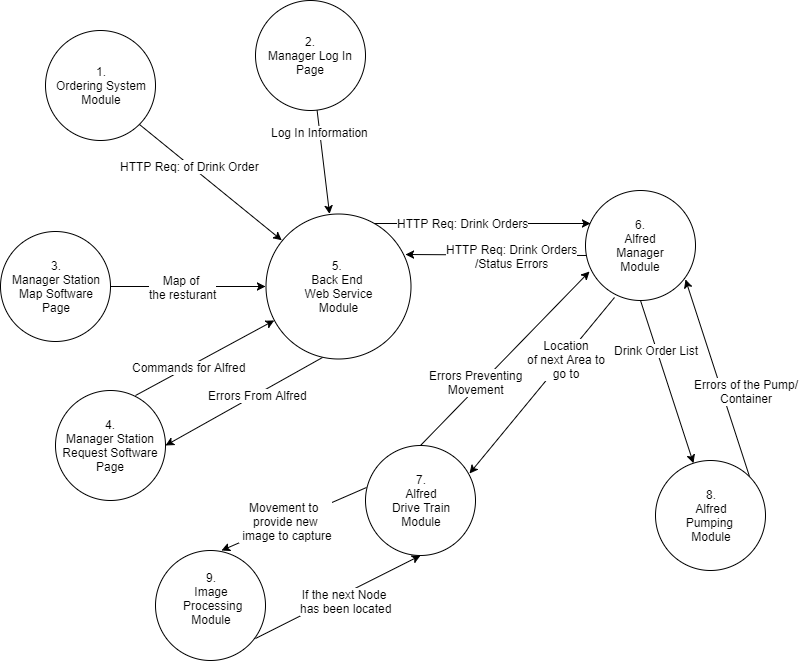
\includegraphics [scale = 0.6] {Figures/SystemComponents.png}
	\caption{Drink Serving Robot System Component Diagram}
\end{figure}
\section{System Variables}

\subsection{Monitored and Controlled Variables}
The following is a list of variables that will be monitored.

\begin{itemize}
	\item $w_{wheel_{left}}$ = Speed of the left sides wheels (rad/s)
	\item $w_{wheel_{right}}$ = Speed of the right sides wheels (rad/s)
	\item $m_{container}$ = Weight of the storage device (kg)
	\item $b_{cupTaken}$ = If the cup has been taken (boolean)
	\item $d_{objects}$ = Set of distances to closest obstacle (m)
	\item $V_{batt}$ = Voltage levels of batteries (V)
	
\end{itemize}

The following is a list of variables that will be controlled
\begin{itemize}
	\item $w_{motor}$ = Speed of the motor (rad/s)
	\item $percent_{dutycycle_{left}}$ = The duty cycle of the left side of the drivetrain (\%)
	\item $percent_{dutycycle_{right}}$ = The duty cycle of the right side of the drivetrain(\%)
	\item $V_{pump}$ = Voltage going to the liquid pumps. (V)
	\item $LED_{drinksignal}$ = Signal of drink that it is ready to be picked up (boolean)
	\item $error_{alfred}$ = Error codes sent from Alfred (unsigned byte)
	\item $error_{drivetrain}$ = Error codes sent from Alfred’s drivetrain module (unsigned byte)
	\item $error_{pump}$ = Error codes sent from Alfred’s pumping system module(unsigned byte)
	\item $Q_{pump}$ = Flow rate of the pump ($m^3/s$)
\end{itemize}

\subsection{Constants}

The following is a list of system constants
\begin{enumerate}
	\item \textbf{$ V_{battMin} $}- The minimum voltage necessary for drivetrain movement (V).
	\item \textbf{$ m_{container_{min}} $}- The minimum weight of liquid necessary for a pump to remain functional. (g)
	\item \textbf{$ m_{drink} $}- The minimum weight of the drink to be considered as ready for the customer. (g)
	\item \textbf{$ t_{timeout} $}- The maximum time Alfred or the ordering application will wait for a message from the server before timing out. (s)
	\item \textbf{$ t_{pumptimeout} $}- The maximum time Alfred will try to pump without noticing a change in the weight of the tank. (s)
	\item \textbf{$ t_{maxpump} $}- The maximum time Alfred will try to dispense a drink within. (s)
	\item \textbf{Steps/Revolution} -  The number of steps within a revolution of the stepper motor (count/rev)
	\item \textbf{$ flow_{pump} $} - The amount of liquid that will be pumped at a specific voltage ($ m^3/s $)
	\item \textbf{$ freq_{bauderate} $} - The  rate at which UART communication will be performed at.
	\item \textbf{$ obstruction_{timeout} $} - The amount of time that Alfred will stop movement due to an object in its path before ruling that there is an obstruction and throwing an error.
\end{enumerate}


\section{Behaviour Overview}
The system is composed of four major parts; the robot, the server, the client application as well as the administrator application. The system will behave in a manner such that the administrator will initially have the capacity to map out the area where the robot will be delivering the drinks. This is done through a graphical interface. Once the administrator creates the map, it will be sent and stored on the server. The administrator will also have the ability to specify the drinks available – which also will be stored on the server. Once the robot is started, it will pull the map from the server to be able to navigate around the area. The client will be able to "order" a drink through the application. This will send the order to the server and will be put in a queue. The robot will be pulling the orders from that queue following a FIFO protocol. As the robot pulls each "order", it will navigate to the table associated with it, and will pour the drinks for that order. The administrator will have the capacity to override the robot at any point, to force its return to "home". Once the drink levels are low in the robot, it will send an "error code" to the server, which will alert the administrator as well.

\section{Component Overview}
\subsection{Ordering System Module}

\subsubsection{Inputs and Outputs}

\textbf{Inputs: } User input defining:
\begin{enumerate}
	\item Number of Orders
	\item List of Ordered Drinks
\end{enumerate}

\textbf{Outputs: } Packaged Information within HTTP Request for:
\begin{enumerate}
	\item Number of Orders
	\item List of Ordered Drinks
	\item Table Number
	\item Identification of the restaurant
\end{enumerate}
\subsubsection{Description}
This module will be used as the user input to take orders of the client. This user input will be taken in by the mobile application based on different button inputs/ radio button selections. These orders are then packaged by the module to be sent to the server based on an HTTP request.

\subsubsection{Timing Constraints}
Timing Constraints are based on the server sending a success signal within $ t_{timeout} $ seconds.

\subsubsection{Initialization}
At startup/new order of the application, it will start a blank order page where the user will be able to add drink orders and use radio buttons to select the desired drink.

\subsection{Manager Login Page Module}

\subsubsection{Inputs and Outputs}

\textbf{Inputs: } 
\begin{enumerate}
	\item String representing the restaurants Username
	\item String representing the restaurant's Password
	\item Indicating which manager component they would like to use
\end{enumerate}

\textbf{Outputs: } 
\begin{enumerate}
	\item Failure message if there is an incorrect information
	\item navigating to the correct page if it was a success.
\end{enumerate}

\subsubsection{Description}
This module is a web based application for the managers to be able to log into the management systems.
\subsubsection{Timing Constraints}
Given optimal networking conditions, the server must respond with $ t_{timeout} $ seconds.

\subsubsection{Initialization}
This will default to a HTML page with no information.


\subsection{Manager Station Map Software Module}

\subsubsection{Inputs and Outputs}

\textbf{Inputs: } User input defining:
\begin{enumerate}
	\item The width of the restaurant
	\item The length of the restaurant
	\item A set of areas in which Alfred can travel to
	\item A set of areas in which contains tables
	\item A set of areas in which Alfred cannot travel to
	\item An area that defines Alfred's home location
\end{enumerate}

\textbf{Outputs: } A text file that contains the following information
\begin{enumerate}
	\item The width of the restaurant
	\item The length of the restaurant
	\item A set of nodes in which Alfred can travel to
	\item A set of nodes in which contains tables
	\item A set of nodes in which Alfred cannot travel to
	\item A node that defines Alfred's home location
\end{enumerate}
\subsubsection{Description}
This module will be used as the user input to create a map where the manager of the restaurant will be able to define the details about the restaurant that will help Alfred with it's navigation to different tables.

\subsubsection{Timing Constraints}
Timing Constraints are based on the server sending a success signal within  $ t_{timeout} $ seconds.

\subsubsection{Initialization}
At startup/new order of the application, it will load in the users map that is associated with their profile. If this is the first time using the application then it will default to a 1x1 map.

\subsection{Manager Station Request Software Module}

\subsubsection{Inputs and Outputs}

\textbf{Inputs: } User input defining:
\begin{enumerate}
	\item calling the robot back to the home base
\end{enumerate}

\textbf{Outputs: } Displaying the following information to the user
\begin{enumerate}
	\item Low liquid levels
	\item Leaking of liquid error
	\item Not pumping error
	\item Not able to move error
	\item Low battery Error
\end{enumerate}
\subsubsection{Description}
This module is used for the manager to determine the state of Alfred from an office as well as being able to override the robot to come back to the home base. 
\subsubsection{Timing Constraints}
One timing constraints are based on the server sending a success signal within  $ t_{timeout} $ seconds. Another constraint is that Alfred will return within the time of $ w_{wheel} $*distance.

\subsubsection{Initialization}
At startup this interface should pull the last status of the robot and display it to the user. If no previous data is found then it will return that there are currently no errors.

\subsection{Back End Web Service Module}

\subsubsection{Inputs and Outputs}

\textbf{Inputs: } 
\begin{enumerate}
	\item HTTP request package with the packaged information for drink orders.
	\item A text file that holds the information about the restaurant map.
	\item HTTP request package with the current list of errors from Alfred
	\item Log in information
\end{enumerate}

\textbf{Outputs: } 
\begin{enumerate}
	\item HTTP request package with the packaged information for drink orders.
	\item A text file that holds the information about the restaurant map.
	\item HTTP request package with the current list of errors from Alfred
	\item Login Success or Fail
	\item Success result for authenticated results. 
\end{enumerate}
\subsubsection{Description}
This module is a server component that will hold account information for different restaurants. This will perform authorize different users to be able to accept different drink requests from the ordering system. It will return the next drink order for the restaurants Alfred robot.
\subsubsection{Timing Constraints}
Given optimal networking conditions, the server must respond with  $ t_{timeout} $ seconds.

\subsubsection{Initialization}
This server will be initialized by a database with one restaurant which will be used for the purposes of testing the system

\subsection{Alfred Manager Module}

\subsubsection{Inputs and Outputs}

\textbf{Inputs: } 
\begin{enumerate}
	\item Text file with a map of the restaurant
	\item A list of drink orders ordered by table
	\item If there is a request to come back to the base
	\item Errors from drive-train system module
	\item Errors from pumping system module
\end{enumerate}

\textbf{Outputs: } 
\begin{enumerate}
	\item Next Drink Order
	\item Next Node to Travel to
	\item Errors from Alfred
\end{enumerate}

\subsubsection{Description}
This module acts as the manager to the different components of Alfred. It will command the drive-train to move to different nodes of the map. The manager will also communicate through UART to the different on board micro-controller for commanding the next drink to the pumping system.
\subsubsection{Timing Constraints}
Given optimal networking conditions, the system must receive a response within  $ t_{timeout} $ seconds. The communication with the pumping system must be done at the specified $freq_{bauderate}$.

\subsubsection{Initialization}
This will assume that there is no requests at startup. It will request from the server asking for the next drink order. If there is no map previously defined within a text file then it will request this as well.

\subsection{Alfred Drive-train Module}

\subsubsection{Inputs and Outputs}

\textbf{Inputs: } 
\begin{enumerate}
	\item Text file with a map of the restaurant
	\item The next node it has to travel to.
	\item $ w_{wheel_{left}} $
	\item $ w_{wheel_{right}} $
	\item $ d_{objects} $ 
	\item $ Marker_{PosX} $
	\item $ Marker_{PosY} $
	\item $ b_{NextMarkerFound} $
\end{enumerate}

\textbf{Outputs: } 
\begin{enumerate}
	\item $ percent_{dutycycle_{left}} $
	\item $ percent_{dutycycle_{right}} $
	
\end{enumerate}

\subsubsection{Description}
This module will provide power to the drive-train of Alfred. It will use the feedback of the left and right encoders and take the error to perform PI control on them. This PI control output will then be translated into a duty cycle for each side to be able to power the DC motors with pulse width modulation. This module will communicate to the image recognition software to receive the position of the next next marker and use this information of where it currently is on its path. This module will use ultrasonic sensors to get a set of distances ($ d_{object} $) to the nearest object to determine if it is safe to continue moving.

\subsubsection{Timing Constraints}
This module will have to deliver speed requirements that of walking speed so that it will be able to serve tables at a timely manner.

\subsubsection{Initialization}
This module will not be started until manager starts the process and initializes the proper information.

\subsection{Alfred Pumping System Module}

\subsubsection{Inputs and Outputs}

\textbf{Inputs: } 
\begin{enumerate}
	\item Drink Order List
	\item $ b_{cuptaken } $
	\item $ m_{containerMin} $
	\item $ m_{drink} $
\end{enumerate}

\textbf{Outputs: } 
\begin{enumerate}
	\item $ LED_{drinksignal} $
	\item $ V_{pump } $
	
\end{enumerate}

\subsubsection{Description}
This module will receive information from the Alfred manager module through UART to receive the next drink order. This will then begin to dispense the specific drink until it has reached $ m_{containerMin} $. It will then show the customer that the drink has been completed by turning on: $ LED_{drinksignal} $. It will then read $ b_{cuptaken} $ from a light sensor to determine if the cup has been taken at which point it will then wait for the next drink cup to get in place and begin pouring. If it is not able to pump liquid, or it is losing fluid when not dispensing, then it will send the appropriate errors through UART back to the manager.

\subsubsection{Timing Constraints}
This module will have to dispense the drink within $ t_{maxpump} $

\subsubsection{Initialization}
This module start by waiting for the manager to send the drink information for the system to pour. All errors within the system will start as false until they have been triggered.
\subsection{Alfred Image Processing Module Module}

\subsubsection{Inputs and Outputs}

\textbf{Inputs: } 
\begin{enumerate}
	\item $ pic_{ceiling} $
\end{enumerate}

\textbf{Outputs: } 
\begin{enumerate}
	\item $ Marker_{PosX} $
	\item $ Marker_{PosY} $
	\item $ b_{NextMarkerFound} $
	
\end{enumerate}

\subsubsection{Description}
This module will receive information from a camera while the drive-train is in motion. This camera will be looking at the ceiling looking for positions of circles that will denote one meter distances set up within a grid around the ceiling of the restaurant. This module will determine if there is a new maker within the image and if so where is the X and Y position of that marker to provide to the drive-train.

\subsubsection{Timing Constraints}
This information must process in time for the drive train to be able to navigate based off of it.

\subsubsection{Initialization}
This module start by the drive-train application.


\section{Normal Operation}
Alfred is a mostly autonomous robot, only requiring human intervention in the event of an error or warning. Alfred will be able to navigate the restaurant by itself, and will serve drinks to tables. Customers will be able to place orders via a mobile application, which will be sent to a server. Orders to serve will be sent to Alfred using a FIFO protocol. Once Alfred has finished with an order, it will be able to request for a new order to serve. Management will be able to recall Alfred to the kitchen at any point using the admin console. In the event of a recall, Alfred will finish the current job and will return to the kitchen afterwards. Management will also be able to create a map of the restaurant and upload it to Alfred, which will give Alfred the means to navigate the restaurant.



\section{Undesired Event Handling}
Alfred will be able to detect undesired behaviours and conditions such as low liquid levels below threshold $ m_{containerMin} $, any issues with pumping liquid, low battery level, leaking liquids, and any blockages in the current path once Alfred has been blocked for a time greater than $ obstruction_{timeout} $. In the event of any error condition, Alfred will send an error code to the kitchen, to alert the staff of the issue. Wherever possible, Alfred will return to the kitchen in an error condition to request a fix. Otherwise, if movement is not possible, the kitchen staff will have to pick Alfred up from the dining room. Along with alerting management of any current errors, Alfred will also be able to indicate whether it is returning to the kitchen or requires pickup.


\end{document}
